\begin{center}
\tikzstyle{block} = [rectangle, draw, fill=blue!20, text width=4em, text centered, rounded corners]
\tikzstyle{line} = [draw, -latex, line width=.3em]

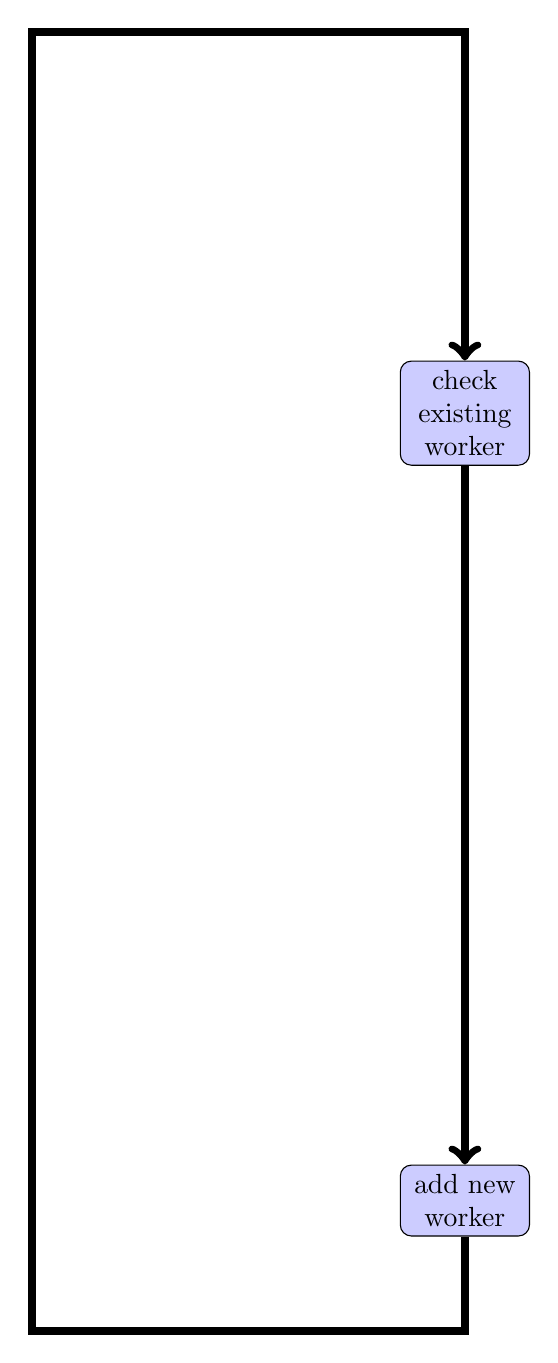
\begin{tikzpicture}[node distance = 2cm, auto]

    % The Main Loop contains
    % * check existing work node
    % * add new transfer

    % PART I 
        \node [block] 
            (part1) {check existing worker};
    % PART II
        \node [block, below of=part1, node distance =10cm] 
            (part2) {add new worker};

    % LINE part1 -> part2
        \path[line,->]
            (part1) -- (part2);
    % LINE part2 -> part1
        \path[line,->]
            (part2.south) |- ++(-5.5,-1.2)
            -- ++(0, 16.5)
            -| (part1.north);

    % in PART I
    % * check status of the worker in DB
    % * check terminate or not
    % * NO
    %   + dump info
    % * Yes
    %   + remove worker from queue
    %   + handle exit code
    %   + update status
\end{tikzpicture}
\end{center}
